For training deep neural networks, we often need expensive hardware if we want to do it on our own. The way to do it these days is to use cloud services such as Google or Amazon to run the machine learning once we have prepared the dataset and the model. We often pay for these services paid by the hour, but they are not expensive as long as we remember to shut them down after use, and only use them when we need to.

Our dataset, however, only contains 55 participants and only a few days of activity measurements for each participant, so using a service to train the model would not be necessary. We decided to train them on one of our personal computers, with an Nvidia GTX 1070. We guess that this GPU will do the job just fine. 
 
\section{Regression}

\begin{figure}
      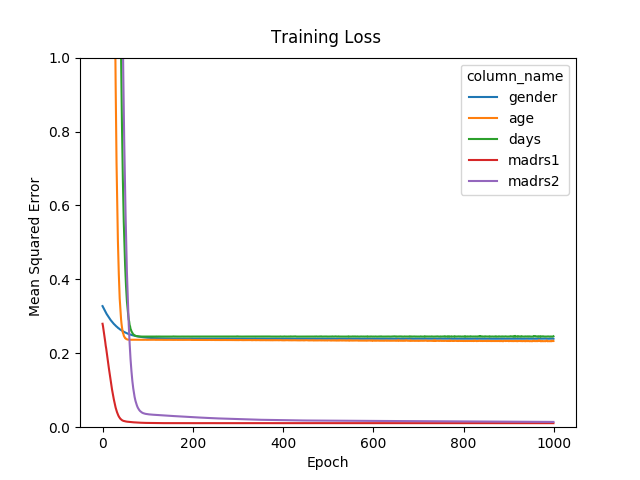
\includegraphics[height=9cm]{img/regression/results_kerasregressor_1k_epochs.png}
      \caption{Regression Training Loss (MSE) by Epoch. The MADRS scores of participants tell more about their condition than gender, age and days.}
      \label{figure:regression_training_loss}
\end{figure}

\begin{figure}
      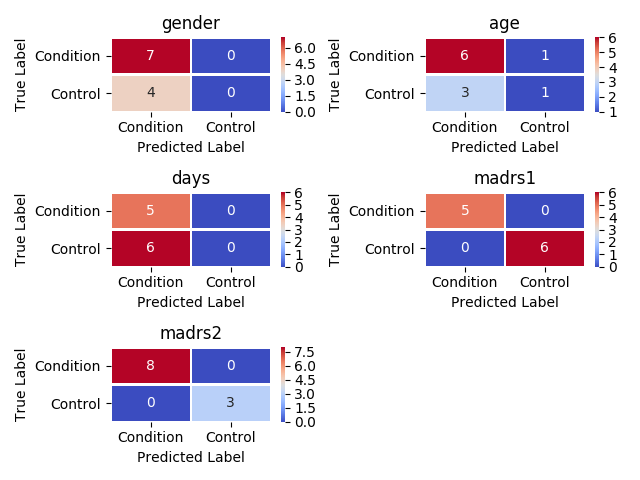
\includegraphics[height=8cm]{img/regression/confusion_kerasregressor_grouped.png}
      \caption{Confusion Matrices for Regression. For both MADRS1 and MADRS2, predictions were perfect.}
      \label{figure:regression_test_confusion}
\end{figure}

We ended up training the regression model \ref{code:regression_model} for 1000 epochs using a batch size of 16. Because of the simplicity of the model, a thousand epochs did not take that much time, and the training loss graph (figure \ref{figure:regression_training_loss}) shows that more epochs will not yield any better results. The loss does not reduce any more after the first 100 epochs for any of the columns. As we said earlier, we wanted the model to predict flawlessly based on the MADRS scores, and the loss results from training these are better than for the other columns. 

We used the \textbf{train\_test\_split} function to create training and testing data, and because of how few rows there are in this dataset, 
we used an 80/20 split for training and testing data. 20\% of the dataset in the test data seemed to be good enough for this experiment because we wanted to train on as many rows as possible. Note that the data elements that were in the test and train splits were different for each column. 

\subsection{Results}

The confusion matrices (figure \ref{figure:regression_test_confusion}) display the results when running the prediction on the test data (and then using it as classification). We said we wanted 100\% on all metrics for the MADRS score columns, and this we can see that this is achieved because the model guessed everything right. The other columns have these performance scores (using \textbf{condition} as positive and \textbf{control} as negative):

\begin{multicols}{2}
\subsection{Accuracy}
$ A = \frac{TP+TN}{TP+TN+FN+FP} $
\\\\
- \textbf{Gender}: $\frac{7+0}{7+0+4+0} = 7/11 \approx 63\%$\\\\
- \textbf{Age}: $\frac{6+1}{6+1+3+1} = 7/11 \approx 63\%$\\\\
- \textbf{Days}: $\frac{5+0}{5+0+6+0} = 5/11 \approx 45\%$\\

\subsection{Precision}
$ P = \frac{TP}{TP+FP} $
\\\\
- \textbf{Gender}:$ \frac{7}{7+0} = 7/7 = 100\%$\\\\
- \textbf{Age}: $\frac{6}{6+1} = 6/7 \approx 86\%$\\\\
- \textbf{Days}: $\frac{5}{5+0} = 5/5 = 100\%$\\

\subsection{Recall}
$ R = \frac{TP}{TP+FN} $
\\\\
- \textbf{Gender}: $\frac{7}{7+4} = 7/11 \approx 63\%$\\\\
- \textbf{Age}: $\frac{6}{6+3} = 6/9 \approx 67\%$\\\\
- \textbf{Days}: $\frac{5}{5+6} = 5/11 \approx 45\%$

\subsection{Specificity}
$ S = \frac{TN}{TN+FP} $
\\\\
- \textbf{Gender}: $\frac{0}{0+0} = 0/0$\\\\
- \textbf{Age}: $\frac{1}{1+1} = 1/2 = 50\%$\\\\
- \textbf{Days}: $\frac{0}{0+0} = 0/0$\\

\end{multicols}

\subsection{F1 Score}
$ F1 = 2 \cdot \frac{P \cdot R}{P + R} $
\\\\
- \textbf{Gender}: $2 \cdot \frac{1 \cdot 0,63}{1 + 0,63} \approx 77\%$\\\\
- \textbf{Age}: $2 \cdot \frac{0,86 \cdot 0,67}{0,86 + 0,67} \approx 75\%$\\\\
- \textbf{Days}: $2 \cdot \frac{1 \cdot 0,45}{1 + 0,45} \approx 62\%$\\

Looking away from the results of \textbf{madrs1} and \textbf{madrs2}, because, the performance scores tell us that the model is good at predicting that someone is in the condition group (precision). Other than that, we cannot learn that much from them. Also, we have undefined specificity for both gender and days because we do not have any predictions for the values required to calculate them. 

However, we learned a lot about machine learning and regression doing this experiment, and we looked at it more like a warmup for the more complex models that we built for the next goals.

\section{1D CNN: Control vs Condition groups}

\subsection{Training and finding the optimal segment length}

Next up was our goal to classify whether a participant belongs to the control group or the condition group. As we said in the section about optimizing the model, the segment length is what we thought was going to impact the result the most. To test this theory, we trained the model to fit input data created with segment lengths of 1, 2, 4, 8, 16, 24, 48 and 96 hours. 

The input data was split using \textbf{train\_test\_split} so that the training data was 80\% of the total and the rest was going to be used for testing after the training was complete. We used 40\% the training data as validation data, which made it easy for us to tell if the model was learning from epoch to epoch or not. 

We did the training for each of the eight different input sets for ten epochs. To keep it simple, we used a batch size of 16 and the Adam optimizer with a default learning rate of 0,001 throughout this experiment. The primary objective here was to find the best segment length to use, and not to train the models to be perfect,  so these hyper-parameters seemed fine for this purpose. Our guess before we started with the experiment was that the more hours of data we used, the better, meaning that 96 hours of data in each segment was going to give us the best model (from what was possible with only ten epochs).

Looking at the history graphs (figure \ref{figure:control_condition_10e}) for how the training went epoch by epoch for each of the experiment's datasets, we noticed that the results were better when increasing the number of hours up to 48, and then it did not seem to be any better for 96 hours. This was the case for both training and testing, as the evaluation graphs (results after testing the model with the test-split) to the right also show straight lines from 48 hours to 96 hours. The question was whether 48 hours was our magic number, or if we just needed to train it more.

To find the best segment length, we needed to experiment with more epochs. We reran the same experiment for 50 epochs, with 48, 72 and 96 hour long segments. However, from the results for that (figure \ref{figure:control_condition_50e}), it is clear that nothing more was achieved with segments longer than 48 hours. 

The classifications for the models trained to fit 48-hour segments you can see in the confusion matrices (figure \ref{figure:control_condition_confusion_matrix_48h}) are close to perfect. The additional 40 epochs of training reduced the false negative classifications by a little bit, which was worth the time in our opinion as we want the value of wrong classifications to be as close to 0 as possible. For this relatively small dataset, we are happy with a classification model with scores above 99\% on all performance metrics previously discussed. 

\begin{figure}
      \begin{multicols}{2}
            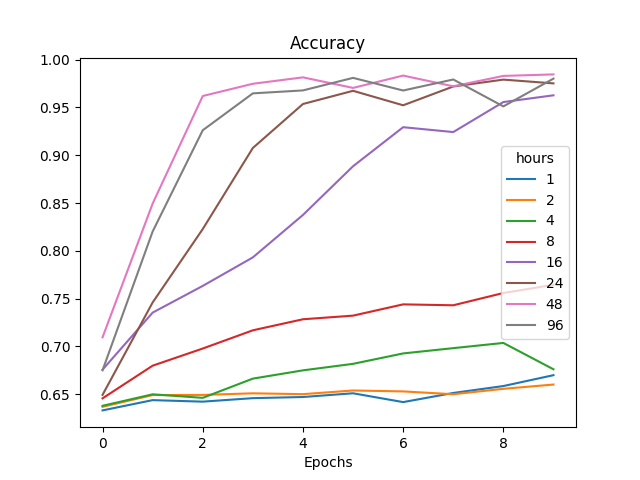
\includegraphics[height=5cm]{img/control_condition/plot_acc_train.png}
            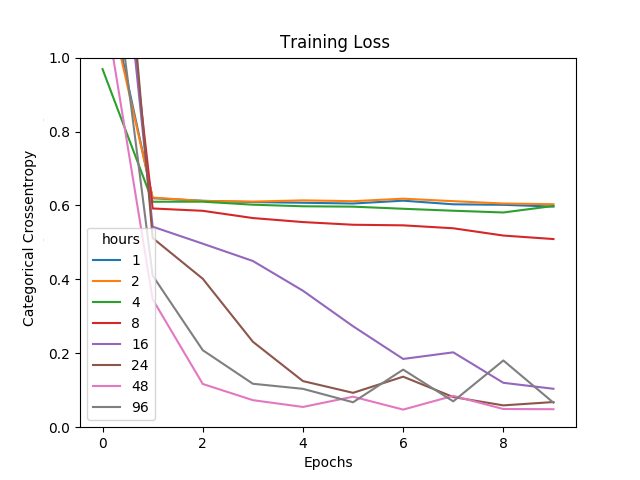
\includegraphics[height=5cm]{img/control_condition/plot_loss_train.png}

            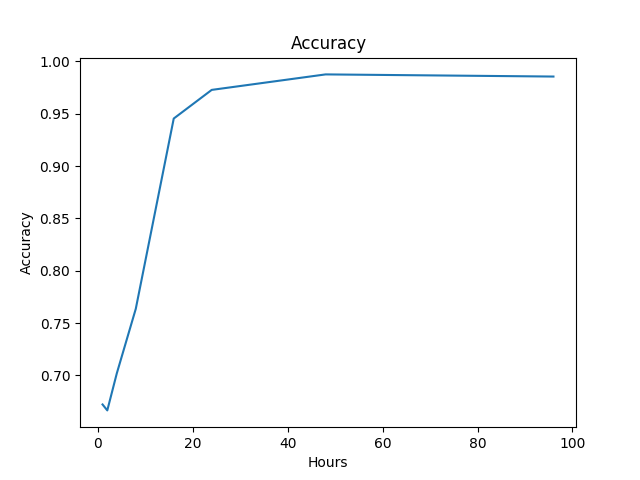
\includegraphics[height=5cm]{img/control_condition/plot_acc_eval.png}
            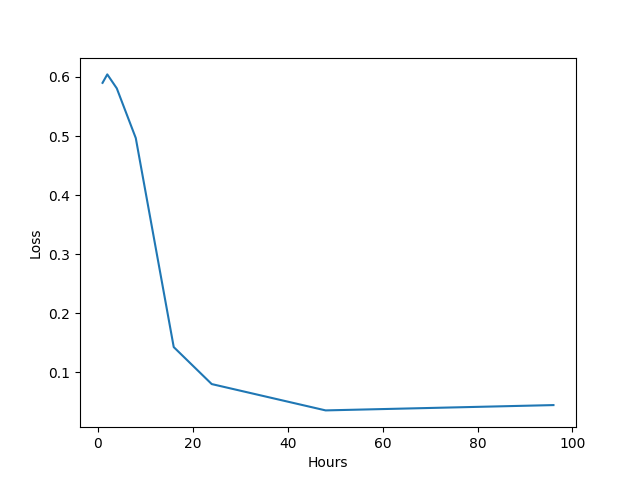
\includegraphics[height=5cm]{img/control_condition/plot_loss_eval.png}
      \end{multicols}
      \caption{Training loss and accuracy is shown on the left side, where we can see that the model performs better with longer segments up to 48 hours. Evaluation results are on the right side, which shows the same improvements but after training is done. The models were trained for 10 epochs.}
      \label{figure:control_condition_10e}
\end{figure}

\begin{figure}
      \begin{multicols}{2}
            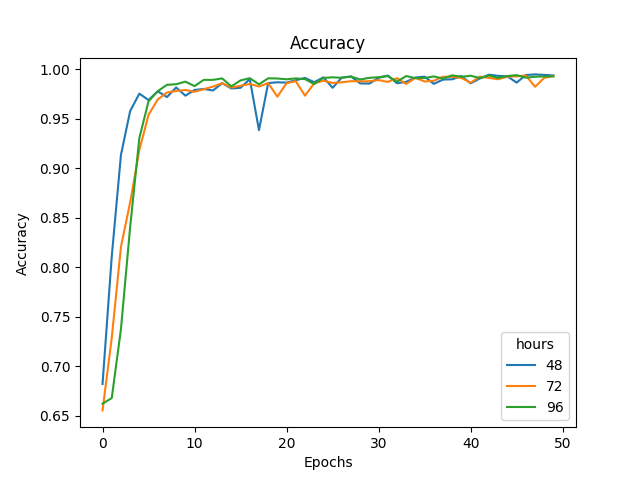
\includegraphics[height=5cm]{img/control_condition/plot_acc_train_50e.png}
            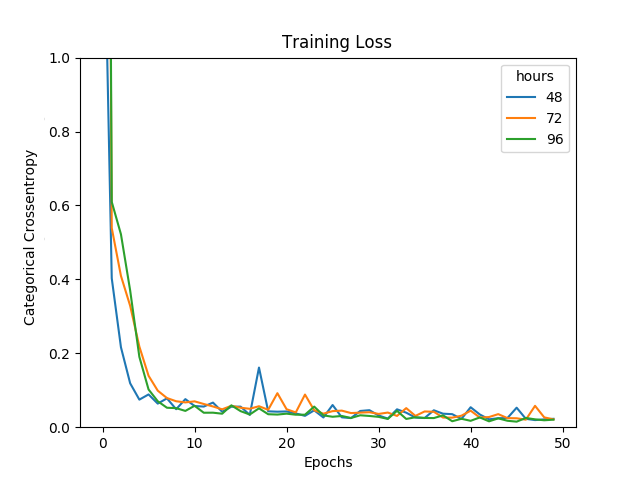
\includegraphics[height=5cm]{img/control_condition/plot_loss_train_50e.png}

            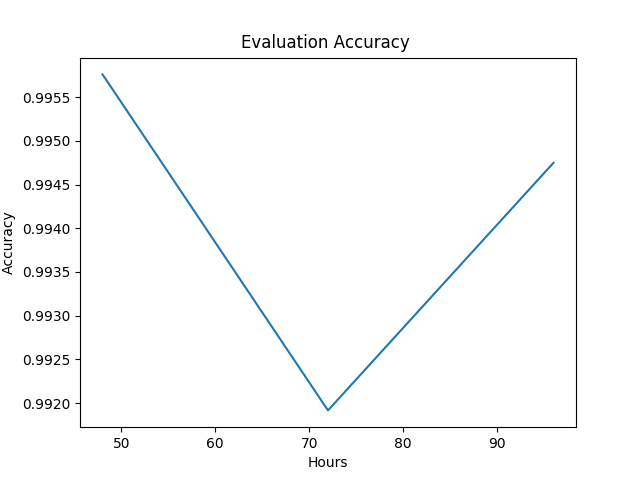
\includegraphics[height=5cm]{img/control_condition/plot_acc_eval_50e.png}
            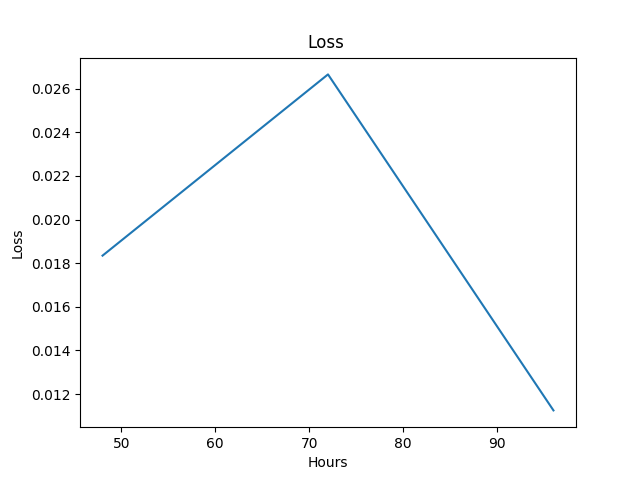
\includegraphics[height=5cm]{img/control_condition/plot_loss_eval_50e.png}
      \end{multicols}
      \caption{Training the models for 50 epochs to find the best segment length. 48 hours was the overall winner with evaluation accuracy very close to 1.0.}
      \label{figure:control_condition_50e}
\end{figure}

\begin{figure}
\begin{center}
      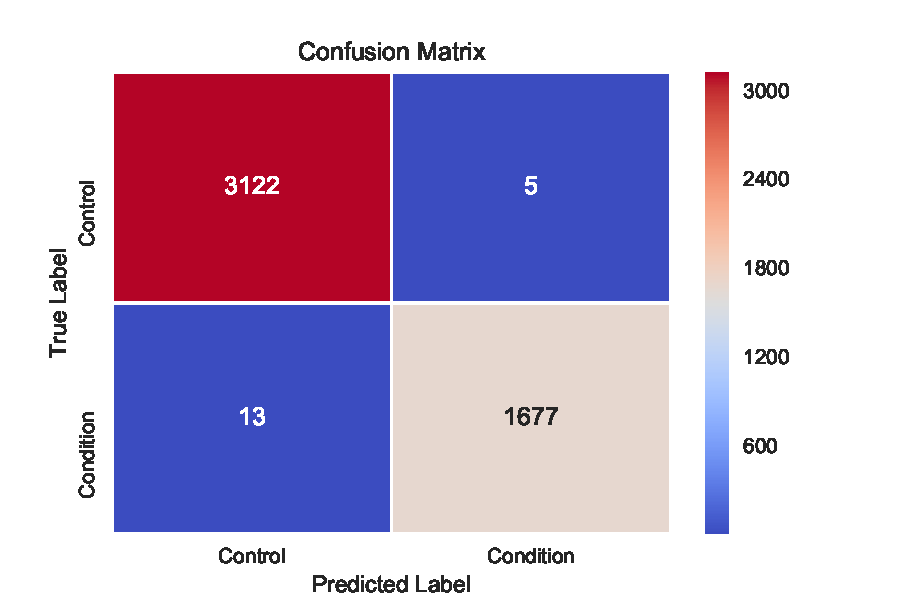
\includegraphics[height=8cm]{img/control_condition/50ep.pdf}
      \caption{Confusion matrix for running the classifier on unseen data. After training the model for 50 epochs, it was able to correctly classify 3122 control group and 1677 condition group segments.}
      \label{figure:control_condition_confusion_matrix_48h}
\end{center}
\end{figure}

%TP   FN   
%FP   TN

\subsection{Performance metrics}

\subsubsection{Accuracy}
$ A = \frac{TP+TN}{TP+TN+FN+FP} = \frac{3122+1577}{3122+1577+5+13} \approx 99,6\%$

\subsubsection{Precision}
$ P = \frac{TP}{TP+FP} = \frac{3122}{3122+13} \approx 0.996$

\subsubsection{Recall}
$ R = \frac{TP}{TP+FN} = \frac{3122}{3122+5} \approx 0.998$

\subsubsection{Specificity}
$ S = \frac{TN}{TN+FP} = \frac{1577}{1577+13} \approx 0.992$

\subsubsection{F1 Score}
$ F1 = 2 \cdot \frac{P \cdot R}{P + R} = 2 \cdot \frac{0,996 \cdot 0,998}{0,996 + 0,998} \approx 0.997 $

\subsection{Cross-validation}

To ensure that our model is not overfitting and did not get lucky when classifying the samples from the testing set, we proceeded to use 3-fold cross-validation. First, we split the dataset in two like before, into a train and test set (80/20 split here as well). Then we generated three folds containing training and validation parts, where for each fold a model was trained to fit the inputs. Each epoch the model was validated against the validation split. After training a model for a fold, we evaluated them by looking at the mean accuracy/loss against the global test split. If the accuracy was still high and the loss was still low, the model would have a good chance of doing correct classifications on unseen data.

\begin{table}[h]
      \begin{center}
          \begin{tabular}{|l|l|l|}
              \hline
              \bfseries Fold & \bfseries Loss & \bfseries Accuracy
              \csvreader[head to column names]{code/logs/control_vs_condition/5f_cv.csv}{}
              {\\\hline\fold & \loss & \accuracy}
              \\\hline
              \bfseries Mean & \bfseries 0.0629539173937511 & \bfseries 0.9809907427163319
              \\\hline
          \end{tabular}
          \caption{3-Fold Cross validation. Overall accuracy was 0.98 and loss 0.06.}
          \label{table:control_condition_5f_cv}
      \end{center}
\end{table}

To make this process quick, we trained the model for each fold only for ten epochs. The goal was to prove consistency in the model and not achieve high performance, so it seemed enough. As one can see in the cross-validation results (table \ref{table:control_condition_5f_cv}), we have a mean loss of $0.06$ and a mean accuracy of $0.98$, which means that the model is consistently correct in most classifications.

\subsection{Leaving one participant out}

However, the above results were for each segment and label, and not specific to any participant. Even though we reduced the chance of overfitting by keeping aside randomized training and testing data, there is a high chance that the training data contains samples from all participants. Garcia-Ceja, E. et al. did \textit{leave one participant out validation} in their paper \cite{GarciaCeja2018_classification_bipolar}, which means that for each participant in the dataset, keep them outside the training data, train on the rest of the participants, then make predictions on the participant that was left out. Each prediction for the left out participant can be different, so to determine the final label they used majority voting (using the most common predicted label). 

We proceeded to do the same experiment as Garcia-Ceja, E. et al., as it would be a good way of comparing our work. For each participant, we generated input data that did not contain any activity data from the participant. Then we created a model and trained it to fit the input data for ten epochs (any more would take too much time considering we had to train 55 models), and made predictions using majority voting. 

\begin{figure}[h]
\begin{center}
      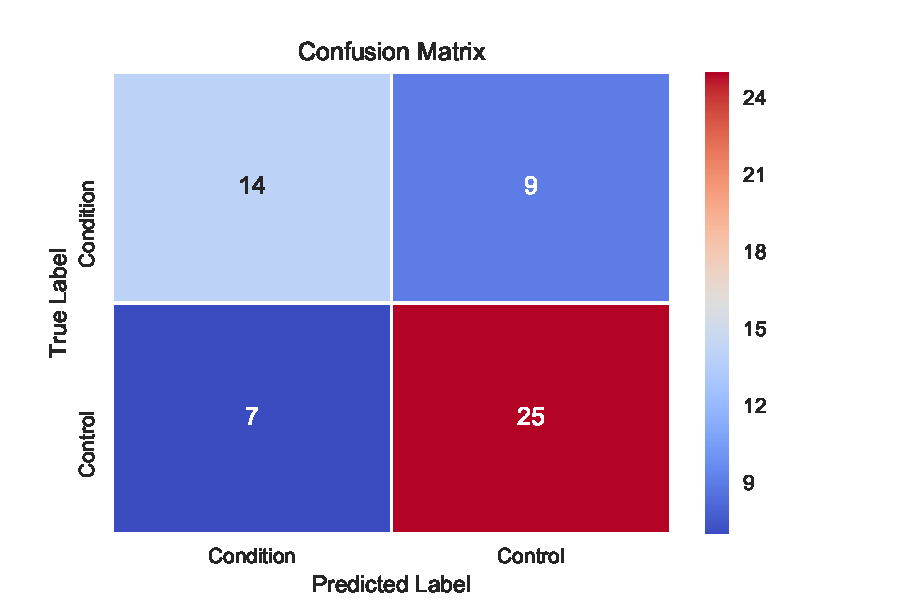
\includegraphics[height=8cm]{img/control_condition/leave_one_out.pdf}
      \caption{Confusion matrix containing detected classes after leave one participant out experiment. The model was best at classifying participants in the control group.}
      \label{figure:control_condition_conf_loo}
\end{center}
\end{figure}

\begin{table}[h]
\begin{center}
      \begin{tabular}{|l|l|l|l|l|l|}
            \hline
            \bfseries Label & \bfseries Accuracy & \bfseries Precision & \bfseries Recall & \bfseries Specificity & \bfseries F1 \\\hline
            Control & 0.71 & 0.74 & 0.78 & 0.61 & 0.76 \\\hline
            Condition & 0.71 & 0.67 & 0.61 & 0.78 & 0.64 \\\hline
            \bfseries Mean & \bfseries 0.71 & \bfseries 0.71 & \bfseries 0.70 & \bfseries 0.70 & \bfseries 0.70 \\\hline
      \end{tabular}
      \caption{Performance metrics for leave one participant out experiment.}
      \label{table:control_condition_performance_loo}
\end{center}
\end{table}

Earlier results were almost perfect, so we expected the results of this experiment to be better than what we can see in the confusion matrix (figure \ref{figure:control_condition_conf_loo}). The model did an excellent job of detecting true negatives (where the correct label and the predicted label is \textit{control}, but the number of false positives and false negatives were a bit too high. We could train the models for more than ten epochs and hope for better results, but we assume it would not be much better because of how little training loss and accuracy changed after the first ten epochs (as seen in the training graph - figure \ref{figure:control_condition_50e}). 

\section{1D CNN: Depression Classes}

\begin{figure}[h]
      \begin{multicols}{2}
            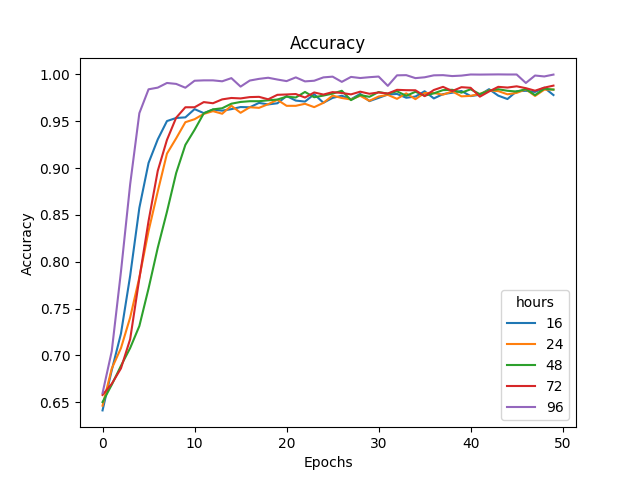
\includegraphics[height=5cm]{img/depression_class/plot_acc_train.png}
            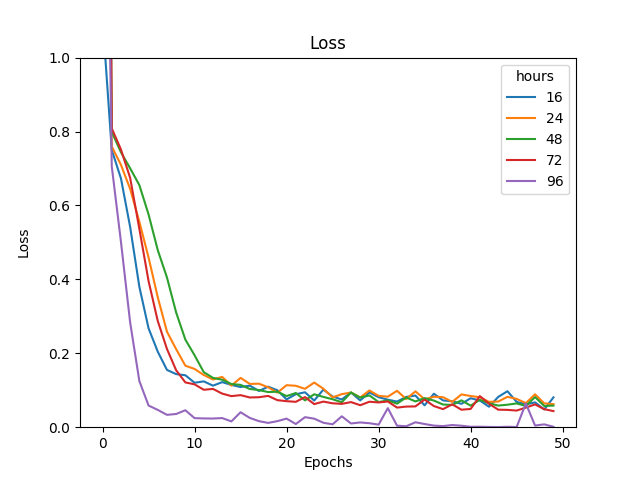
\includegraphics[height=5cm]{img/depression_class/plot_loss_train.png}

            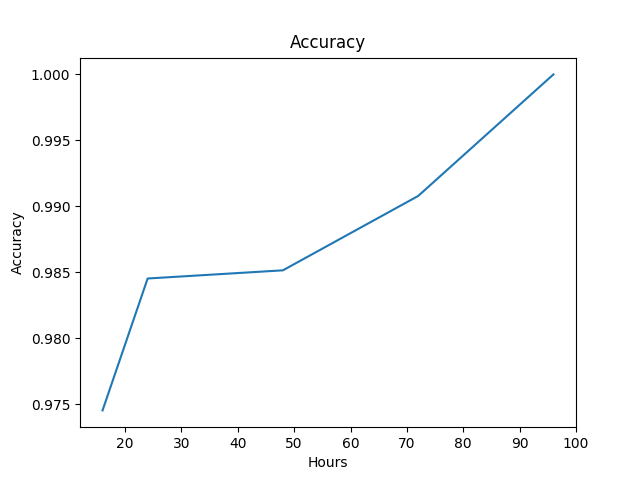
\includegraphics[height=5cm]{img/depression_class/plot_acc_eval.png}
            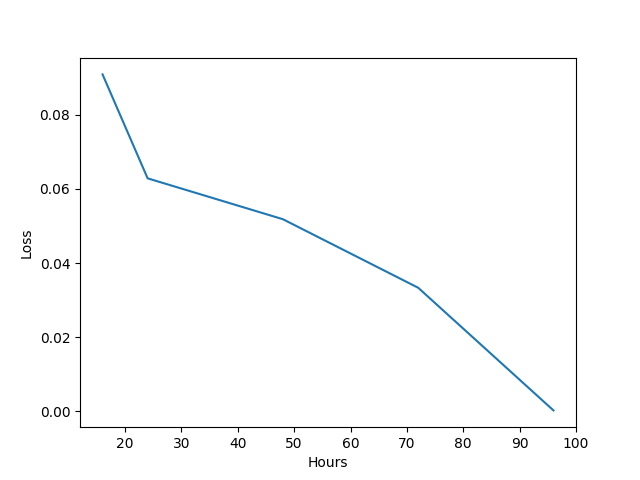
\includegraphics[height=5cm]{img/depression_class/plot_loss_eval.png}
      \end{multicols}
      \caption{Experimenting with segment lengths for classifying depression classes. After 50 epochs we can see that loss and accuracy continues to be better with longer segments.}
      \label{figure:depression_class_50e}
\end{figure}

\begin{figure}[h]
\begin{center}
      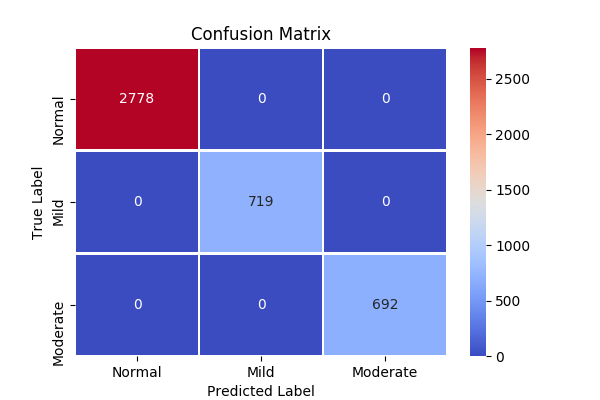
\includegraphics[height=8cm]{img/depression_class/conf_5760_60_50_32.png}
      \caption{After training the model on 96 hour long segments for 50 epochs, classification on test-data segments is perfect.}
      \label{figure:depression_class_confusion_matrix_96h}
\end{center}
\end{figure}

\subsection{Training and finding the optimal segment length}

The next neural network we trained was for classifying how depressed the participants were. Depression classes are, as we said before, 
based on their MADRS score which is 0 for participants in the control group and differs between 11 and 28 in the condition group (figure \ref{figure:demographics}). We labeled participants with MADRS score 0 as not depressed, between 11 and 19 as mildly depressed, and above 20 as moderately depressed. 

Using what we previously discovered from classifying control vs. condition groups, we knew how we wanted to achieve this goal. First, find the optimal segment length, then use the best segment length in cross-validation, and guarantee that the performance is consistent. 

In the previous experiment, there was a clear threshold after segment lengths of 24 hours where the performance did not improve that much if increased more (figure \ref{figure:control_condition_10e}). The results were just a little bit better for 48 than 24 hours and worse for longer segments. The question was whether the threshold existed for depression classes also, or if we could use longer segments to achieve better results.

We experimented the same way as before, except that we went straight for 50 epochs and skipped the shortest segments of 1, 2, 4 and 8 hours, as we were positive these segments would not be any good. We proceeded to train segment lengths of 16, 24, 48, 72 and 96 hours. Looking at the training and testing graphs (figure \ref{figure:depression_class_50e}), we can see that the results for 96-hour segments were outstanding. We achieved an accuracy of 100\% on the testing set. The confusion matrix (figure \ref{figure:depression_class_confusion_matrix_96h}) shows not a single error in classification. 
 
\subsection{Cross-validation}

\begin{table}[h]
\begin{center}
      \begin{tabular}{|l|l|l|}
            \hline
            \bfseries Fold & \bfseries Loss & \bfseries Accuracy
            \csvreader[head to column names]{code/logs/depression_class/cv.csv}{}
            {\\\hline\fold & \loss & \accuracy}
            \\\hline
            \bfseries Mean & \bfseries 0.032561721418313254 & \bfseries 0.990689902124612
            \\\hline
      \end{tabular}
      \caption{3-Fold Cross validation for this experiment to verify consistency of the model. All three folds perform well.}
      \label{table:depression_class_cv}
\end{center}
\end{table}

To make sure this was not just lucky, we needed to cross-validate here as well. We split the dataset into a training and testing set (80\%/20\%), then did three-fold cross-validation on the training set, just as before. If all three folds had similar accuracy and loss, and the mean values were good (close to 1.0 for accuracy and close to zero for loss), we had achieved a consistent model, and the model would be fit perfectly, at least for the 55 participants in the dataset. 

We trained the three models for 15 epochs each. We knew that was not enough to give us 1.0 accuracy (need around 50 epochs for that), but we aimed for somewhere around 0.98-0.99 for all folds. Looking at the cross-validation results (table \ref{table:depression_class_cv}), we can see that the lowest accuracy was 0.985 and the highest was 0.998. The mean accuracy for all three folds was 0.99, which is what we wanted to see. 

\subsection{Leaving one participant out}

\begin{figure}[h]
\begin{center}
      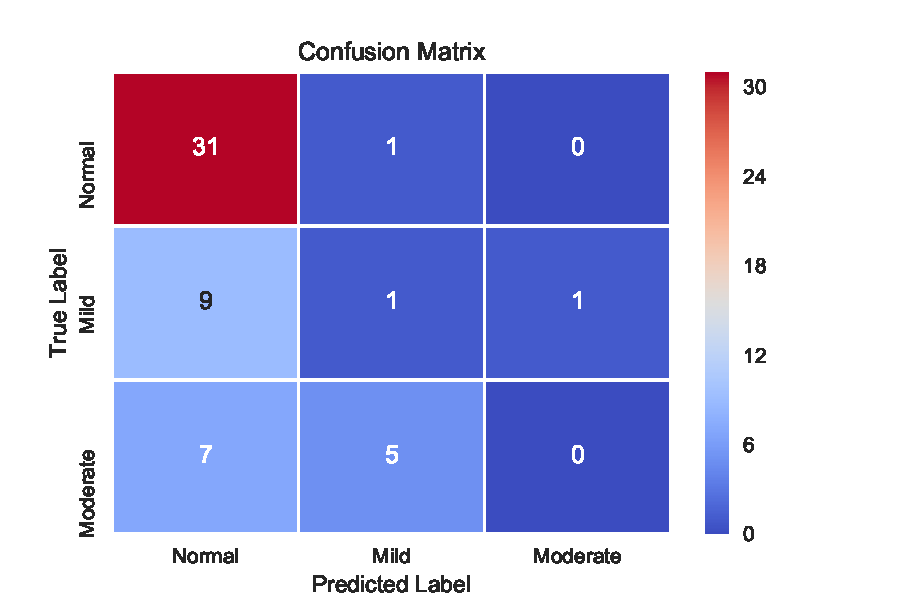
\includegraphics[height=8cm]{img/depression_class/leave_one_out.pdf}
      \caption{Confusion matrix containing detected classes after leave one participant out experiment. The model was only good for detecting normal participants.}
      \label{figure:depression_class_conf_loo}
\end{center}
\end{figure}

\begin{table}[h]
\begin{center}
      \begin{tabular}{|l|l|l|l|l|l|}
            \hline
            \bfseries Label & \bfseries Accuracy & \bfseries Precision & \bfseries Recall & \bfseries Specificity & \bfseries F1 \\\hline
            Normal & 0.69 & 0.66 & 0.97 & 0.30 & 0.79 \\\hline
            Mild & 0.70 & 0.14 & 0.09 & 0.86 & 0.11 \\\hline
            Moderate & 0.76 & 0.0 & 0.0 & 0.98 &  \\\hline
            \bfseries Mean & \bfseries 0.72 & \bfseries 0.30 & \bfseries 0.35 & \bfseries 0.71 & \bfseries 0.30 \\\hline
      \end{tabular}
      \caption{Performance metrics for leave one participant out experiment.}
      \label{table:depression_class_performance_loo}
\end{center}
\end{table}
We repeated the same experiment from the end of the previous goal, where we trained on all participants except one that we left for testing afterward. Looking at the confusion matrix \ref{figure:depression_class_conf_loo}, the model seemed to be good at detecting non-depressed participants (F1-score of 0.79), and terrible at everything else (F1-score of 0.11 for mild depression and the model did not detect any participant with moderate depression). Overall, we calculated a mean F1-score of 0.30 for this model (see table \ref{table:depression_class_performance_loo}). 


\section{1D CNN: MADRS Score Prediction}
Now that we have models for classifying both whether a participant belongs to the control group or the condition group and how depressed participants are, we can get started on our last goal which is predicting the MADRS score of our participants. 

Training a prediction model is significantly more computationally heavy than training a classification model. We noticed this as soon as we started the training when the loss started on around 100 which is very high, and prediction on test data after a few epochs was poor. In classification, we were used to training and validation loss between 1 and 0 and reaching a high accuracy after only a few epochs. We had to train for some epochs to compare segment lengths, which would only show which are best in the first epochs.

\subsection{Segment length}
The plan was to perform 100 epochs of training for different segment lengths. We used the same segment lengths as we did for the previous model: 16, 24, 48, 72 and 96 hours. Since the two classification experiments had a different optimal segment length, it was an interesting question whether this was the case for regression as well. 

After finding the best segment length, we used the one with the most promising results to train the model for a more extended period. We wanted to see how good performance we could achieve if we increased the number of epochs by a lot and let it learn overnight. 

\subsection{Cross-validation}
Before training the model to be as perfect as possible, we did cross-validation to check its consistency. Just as we had done before, we performed 3-fold cross-validation. For each fold, we trained the model for 100 epochs to fit the corresponding training data and validated on the corresponding validation data. Then, after a model had completed its training, it was evaluated against the global test data (same procedure as the two previous experiments). Finally, the Mean Squared Error for each fold was saved and compared with other folds to see how they averaged. Table \ref{table:madrs_prediction_cv} contains the cross-validation results, and it seems that the model is consistent.


\begin{table}[h]
\begin{center}
      \begin{tabular}{|l|l|l|}
            \hline
            \bfseries Fold & \bfseries Mean Squared Error
            \csvreader[head to column names]{code/logs/madrs_prediction/cv.csv}{}
            {\\\hline\fold & \mse}
            \\\hline
            \bfseries Mean & \bfseries 31.398445818687225
            \\\hline
      \end{tabular}
      \caption{3-Fold Cross validation for the prediction model. Only small variation between the folds tells us that the model is consistent enough.}
      \label{table:madrs_prediction_cv}
\end{center}
\end{table}

\begin{figure}[h]
      \begin{multicols}{2}
            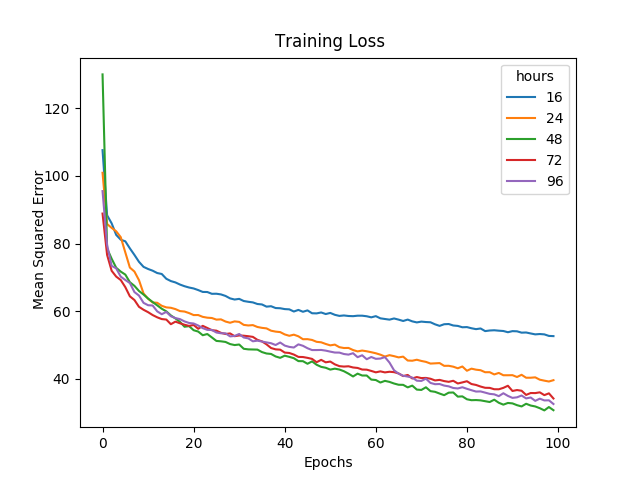
\includegraphics[height=5cm]{img/madrs_prediction/plot_loss_train.png}
            \vfill
            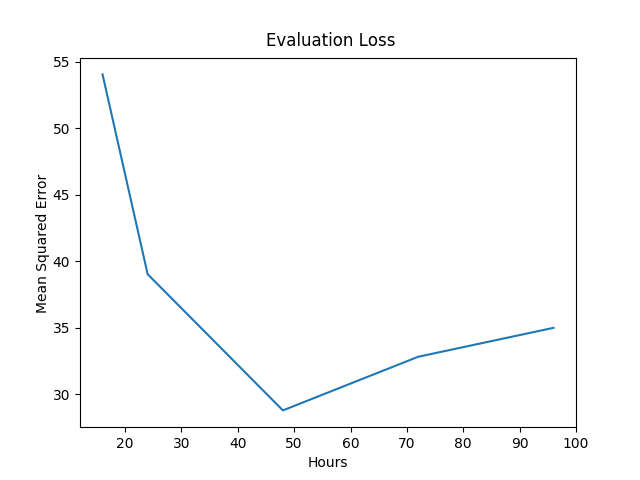
\includegraphics[height=5cm]{img/madrs_prediction/plot_loss_eval.png}
      \end{multicols}
      \caption{Training the MADRS prediction model for 100 epochs with different segment lengths. The model trained on 48-hour segments performed best.}
      \label{figure:madrs_prediction_50e}
\end{figure}

\subsection{Hyper-parameters}
\begin{figure}[h]
\begin{center}
      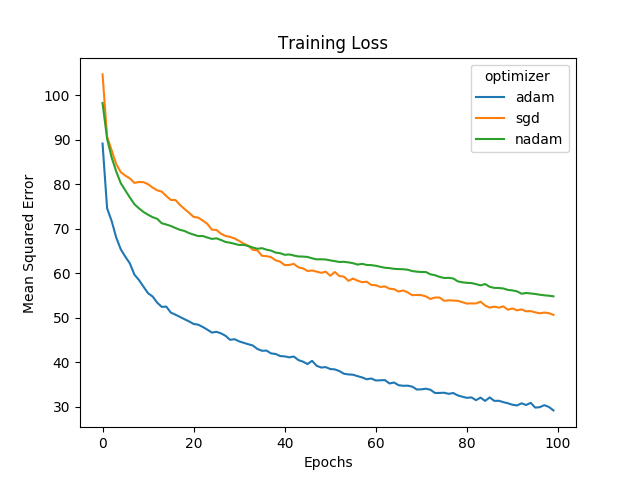
\includegraphics[height=7cm]{img/madrs_prediction/optimizers.png}
      \caption{Training the models with 48-hour segments for 100 epochs, comparing different optimizers. The Adam optimizer performed significantly better than SGD and Nadam.}
      \label{figure:madrs_prediction_optimizers}
\end{center}
\end{figure}

\noindent From the training and evaluation graphs (figure \ref{figure:madrs_prediction_50e}), it seemed like the way to go was 48-hour segments. We don't know what's best for training 
the model further, but this was what we settled on using. 

Also, unlike the classification experiments, we experimented more with hyper-parameters. The Adam optimizer with default learning rate did the job for classification, 
but now that we had to train for thousands of epochs, these parameters had the potential to affect the results by a lot. 
We proceeded to compare three different optimizers: Adam, SGD, and Nadam. We had to change the learning rate to get SGD to work 
(the default which is 0.01 \cite{keras_docs} resulted in NAN MSE for some reason). All optimizers were set to use a learning rate of 0.0001. 
The optimizer comparison graph (figure \ref{figure:madrs_prediction_optimizers}) shows that Adam was the best choice for MADRS prediction as well. 


\subsection{Training the model}
To summarize, this model was trained to fit segments of length 48 hours (2880 minutes). It was trained with the optimizer Adam using a learning rate of 0.0001. We did not change the batch size; we kept this at 16. We split the dataset into 60\% training data and 40\% testing data. Based on the time it took to train each of the 100-epoch experiments, we calculated that around 2700 epochs of training would be a realistic amount.

When we checked for results the next day, we could see the training had resulted in a mean squared error approximately at 4.0 (on validation data). The training graph (figure \ref{figure:madrs_prediction_history}) shows that further training would not necessarily give any better results. Predictions on the test data (figure \ref{figure:madrs_prediction_testset}) looked very promising. The graph shows correct MADRS scores in the x-axis and the predicted MADRS scores in the y-axis. Each blue dot is a prediction, and the dotted black line is a linear guideline for the perfect predictions (where the predicted and correct scores are the same). 

\begin{figure}[h]
\begin{center}
      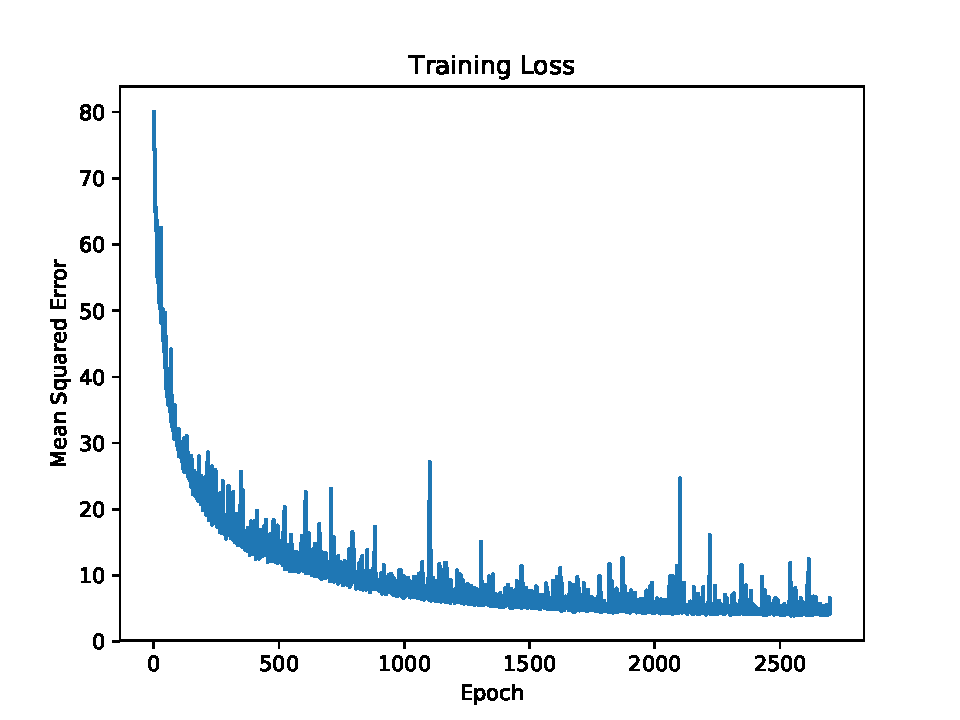
\includegraphics[height=8cm]{img/madrs_prediction/train_history.pdf}
      \caption{MADRS Prediction: Training history throughout 2700 epochs. The MSE is approximately 4.0 after 2000 epochs.}
      \label{figure:madrs_prediction_history}
\end{center}
\end{figure}

\begin{figure}[h]
\begin{center}
      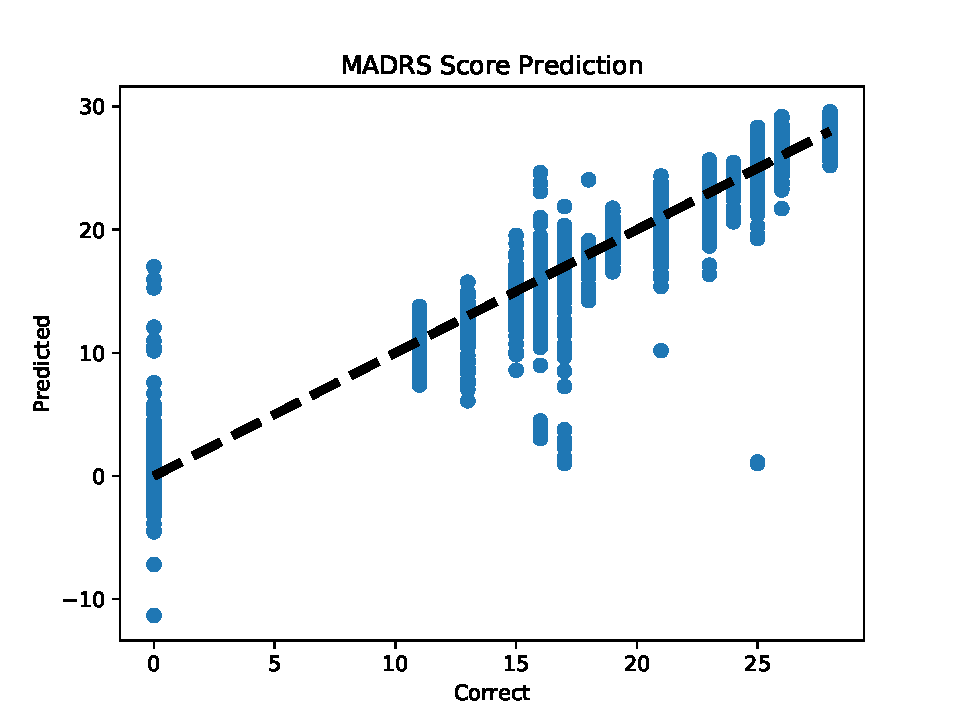
\includegraphics[height=8cm]{img/madrs_prediction/predictions.pdf}
      \caption{Running the MADRS prediction model on unseen segments. The predictions are not perfect, but they somewhat follow the black dotted line (where predictions and correct MADRS scores are the same).}
      \label{figure:madrs_prediction_testset}
\end{center}
\end{figure}

